

\chapterquote{We can only measure what Nature sends us}{Jim Cronin}  


%%%%%% Párrafo check%%%%%%
La parte superior de la atmósfera terrestre está siendo constantemente bombardeada con partículas provenientes del espacio, con energías de los $10^{10}\,$eV para arriba en la región de Cuyo. Estas partículas son conocidas como rayos cósmicos (RC) y han sido descubiertas en 1911 por Victor Hess. Aunque el área lleva tiempo siendo estudiada, los mecanismos que producen los RCs y las zonas del espacio donde se originan los mismos siguen siendo investigadas por distintos experimentos.  A partir del 2004, el Observatorio Pierre Auger ha detectado rayos cósmicos con el objetivo de estudiar su origen. Un análisis adecuado de los eventos registrados es necesario para estudiar las posibles fuentes de rayos cósmicos, además de su composición y espectro de energía.
%%%%%%%%%%%%%%%%%%%%%%%%%%%%%

%%%%%%%%%%%Check%%%%%%%%%%%%%
Un aspecto estudiado por varios trabajos \cite{collaboration2013pierre} \cite{data} es la distribución de las direcciones de arribo de los rayos cósmicos. Estas direcciones son prácticamente isotrópicas salvo variaciones pequeñas alrededor de la media, por lo que es importante tener en cuenta todos los efectos que pueden ser fuentes de modulación espuria sobre los datos. Un ejemplo claro de una modulación que no aporta información sobre las anisotropías es la modulación del clima.
%%%%%%%%%%%%%%%%%%%%%%%%%%%%%

%%%%%%%%%%%%Check%%%%%%%%%%%%%%%%%
Este trabajo consiste en el análisis de las direcciones de arribo de los rayos cósmicos de ultra alta energía registrados por el Observatorio Pierre Auger. En el mismo se estudia la modulación del clima sobre los eventos medidos por los detectores de superficie, y además se estudian las anisotropías a grandes escalas angulares para distintos rangos de energía desde 0.25 EeV.  

%%%%%%%%%%%%%%%%%%%Check%%%%%%%%%%%%%%%%%%%%%%%%%%%%
Los distintos capítulos de este trabajo están organizados para introducir los rayos cósmicos, mencionar brevemente algunas características del Observatorio Pierre Auger y describir los métodos utilizados para el estudio de los rayos cósmicos, para luego presentar los resultados del análisis sobre la modulación del clima de la señal medida por el Observatorio, y por último reportar los resultados de las amplitudes y fases de las modulaciones sobre la tasa de eventos para distintos rangos de energía.
%%%%%%%%%%%%%%%%%%%%%%%%%%%%%%%%%%%%%%%%%%%%%%%%%%%%
\section{Rayos cósmicos}
%%%%%%%%%%%%%%%%%%%%%%Check%%%%%%%%%%%%%%%%%%%%%%%%%%
Los rayos cósmicos (CRs) fueron descubiertos en 1911 por Victor Hess \cite{hess1912}. Los mismos son partículas que llegan a la Tierra desde el espacio como  electrones, positrones, rayos gamma entre otros, además de núcleos atómicos. En 1962, el experimento \emph{Volcano Ranch} detectó un evento asociado a un CR con energía cercana a $10^{20}\,$eV. Posterior a esta medición, otros experimentos encontraron más eventos por encima de esta energía. 
%%%%%%%%%%%%%%%%%%%%%%%%%%%%%%%%%%%%%%%%%%%%%%%%%%

%%%%%%%%%%%%%%%%%%%Check%%%%%%%%%%%%%%%%%%%%%%%%%%%%%%%
A pesar de que han sido medidos y estudiados en experimentos alrededor del mundo, el origen de los CRs es incierto. Las partículas con energía por encima de $10^{18}\,$eV se conocen como rayos cósmicos de ultra alta energía (UHECRs) y son las partículas con más energía en  medidas hasta momento. Las direcciones de arribo de los UHECRs son casi isotrópicas  \cite{collaboration2013pierre} \cite{data} y se cree que son de origen extra-galáctico, es decir, que no fueron producidos dentro de la Vía Láctea. Esto se debe a que los campos magnéticos galácticos no pueden confinarlos, además que la distribución de sus direcciones de arribo es aproximadamente uniforme en el cielo, sin correlación significativa con el plano o el centro galáctico. 
%%%%%%%%%%%%%%%%%%%%%%%%%%%%%%%%%%%%%%%%%%%%%%%%%%

%%%%%%%%%%%%%%%%%%%%Check%%%%%%%%%%%%%%%%%%%%%%%%%%%%%%
Para estudiar los CRs, se disponen de tres observables principales: el espectro, la composición y la anisotropía. El espectro se refiere a la distribución de energía de los CRs detectados, la composición es la distribución de masas nucleares, es decir que elementos y en que proporción se encuentran en los CRs, y el tercero, la anisotropía, es la distribución de las direcciones de arribo a distintas energías.
%%%%%%%%%%%%%%%%%%%%%%%%%%%%%%%%%%%%%%%%%%%%%%%%%

\section{Espectro de energías}
%%%%%%%%%%%%%%%%%%% check%%%%%%%%%%%%%%%%%%%%%%%%%%
Los mecanismos de interacción con el medio de protones y núcleos de origen extra-galáctico y su relevancia en la propagación fueron predichos por Greisen \cite{greisen1966end}, e independientemente por Zatsepin y Kuzmin \cite{zatsepin1966upper} tras el descubrimiento de la radiación cósmica de fondo (CMB). Durante la propagación  de estas  partículas por el medio extra-galáctico, las mismas sufren una pérdida de energía debido a la expansión del universo. Este el principal mecanismo de pérdida de energía para protones de $E < 2\times 10^{18}\,$eV y núcleos de $E/A < 0.5\times 10^{18}\,$eV. Además estos RCs de origen de extra-galáctico, pierden energía al interactuar con los fotones del  CMB.  Estos procesos de pérdida de energía se conocen como el efecto GZK.
%%%%%%%%%%%%%%%%%%%%%%%%%%%%%%%%%%%%%%%%%%%%%%%%%

%%%%%%%%%%%%%%%%%%No Check%%%%%%%%%%%%%%%%%%%%%%%%%%%%%%%
En la Fig.\,\ref{fig:spectra} se presenta el espectro de los rayos cósmicos medidos por distintos experimentos. La figura fue extraída del trabajo \cite{PGD}, en la misma los datos fueron multiplicados por $E^{2.6}$ para resaltar los cambios en la forma del espectro. Considerando que los CRs de energías por debajo de $\sim  10^{17}\,$eV son probablemente en su mayoría de origen galáctico, la rodilla que marca el cambio de pendiente alrededor de $\sim 3\times10^{15}\,$eV podría reflejar una transición en el origen de los CRs. La rodilla indicaría el límite donde los procesos que aceleran los protones han alcanzado su energía máxima. El experimento de Kascade-Grande ha reportado una segunda rodilla cercana a $8\times10^{16}\,$eV, que podría corresponder al límite de aceleración de primarios más pesados \cite{PGD}.
%%%%%%%%%%%%%%%%%%%%%%%%%%%%%%%%%%%%%%%%%%%%%%%%%

\begin{figure}[H]
	\centering
	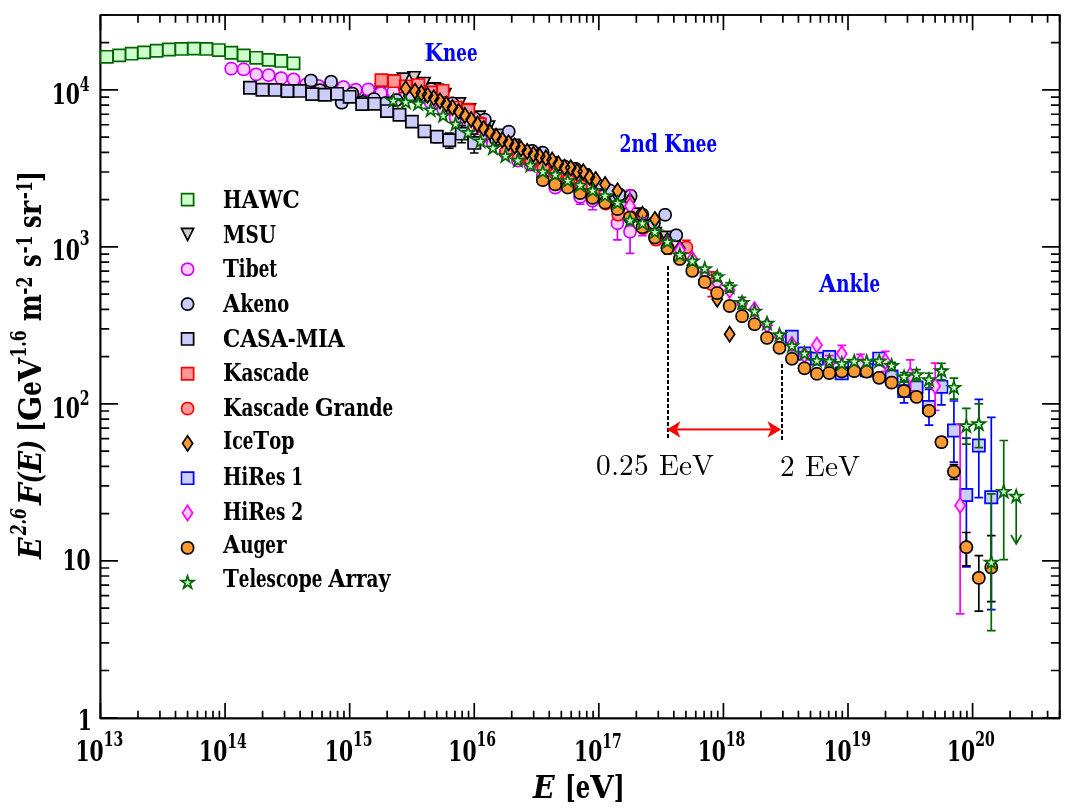
\includegraphics[width=0.7\textwidth]{auger_spectrum_v3.png}
	\caption{Espectro de rayos cósmicos medidos mediante lluvias atmosféricas en función de la energía $E$. Figura obtenida del \emph{Particle Data Group} \cite{PGD}.}
	\label{fig:spectra}
\end{figure}

%%%%%%%%%%%%%%%%%%%%%Check%%%%%%%%%%%%%%%%%%%%%%%%%%%%
Hay diversas teorías detrás del tobillo alrededor de $5 \times 10^{18}\,$EeV en la Fig\,\ref{fig:spectra}. Una teoría dice que el mismo se debe a que una población con un espectro más duro está superando a otra con espectro más blando, por ejemplo un flujo extra-galáctico empieza a dominar sobre un flujo galáctico \cite{bird1994cosmic}. Otra explica que el cambio de la forma de la curva se debe a la pérdida de energía de los protones extra-galácticos, debido al proceso $p\,\gamma \rightarrow\,e^+\,+\,e^-$ conocido como producción de pares con el CMB \cite{berezinsky2006astrophysical}. Una fuerte supresión del espectro para energías por encima de $5\times 10^{19}\,$eV se espera para protones debido a la foto-producción de piones por interacciones con el CMB y para núcleos pesados por foto-desintegración por interacciones con el fondo de radiación infrarrojo. La supresión observada podría deberse a estos procesos, a que las fuentes alcanzan la máxima energía de aceleración o a una combinación de ambos efectos. 
%El proceso para núcleos más pesado es el de foto-desintegración. Para RCs con energías  mayores  a $\nicefrac{E}{A} \geq 6\times 10^{19}\,$eV, el proceso dominante en la pérdida de energía están asociados al efecto GZK \cite{taborda}.
%%%%%%%%%%%%%%%%%%%%%%%%%%%%%%%%%%%%%%%%%%%%%%%%

%%%%%%%%%%%%%%%%%%%Check%%%%%%%%%%%%%%%%%%%%%%%%%%%%%
El flujo de los rayos cósmicos $\Phi$ en función de la energía $E$ puede aproximarse a una ley de potencias que tiene una forma del siguiente tipo
\begin{equation}
	    \frac{d\Phi}{dE} \propto \ E^{-\gamma}   \label{eq:expresion1}
\end{equation}
donde $\gamma$ se lo denomina índice espectral. Este valor varía ligeramente para distintos rangos de energía. Para el rango de energía estudiado en este trabajo, entre 0.25 EeV y 2 EeV como se indica en la Fig.\ref{fig:spectra}, el valor aproximado del índice espectral es $\gamma= 3.27 \pm 0.05$ \cite{data}.


\section{Lluvias atmosféricas extendidas}

%%%%%%%%%%%%%%%%%%%Check%%%%%%%%%%%%%%%%%%%%%%%%%%%%%

{Por encima de una energía de $10^{14}\,$eV, los RCs que llegan a la atmósfera pueden interactuar con las moléculas de la misma,  y así producir cascadas de partículas secundarias. Dependiendo de la energía del primario, es decir el RC que generó la lluvia, estas partículas pueden ser medidas usando detectores sobre la superficie de la Tierra. Esta cascada es conocida como lluvia atmosférica extendida o \emph{EAS} y está compuesta por una componente electromagnética, que consiste en electrones, positrones y fotones, una componente muónica y una componente hadrónica. Las partículas secundarias cargadas también pueden excitar moléculas de nitrógeno en el aire que producen fotones de fluorescencia y pueden ser observados por telescopios durante noches claras.}

%%%%%%%%%%%%%%%%%%%Check%%%%%%%%%%%%%%%%%%%%%%%%%%%%%
El momento transversal que adquieren las partículas secundarias en el proceso de dispersión a través de la atmósfera es tal que los secundarios se dispersan sobre un área de gran tamaño. Por ejemplo, para energías mayores a 10$\,$EeV,  la lluvia puede llegar a cubrir más de 25\,km$^2$. 

%%%%%%%%%%%%%%%%%%%Check%%%%%%%%%%%%%%%%%%%%%%%%%%%%%
El desarrollo de la lluvia puede describirse mediante la profundidad atmosférica $X(L)$, definida como la masa de aire por unidad de área que atravesó una partícula en su dirección de propagación tras recorrer una distancia $L$, 
\begin{equation}
	X(L)= \int_0^L dx \rho(x)
\end{equation}
donde $\rho$ es la densidad del aire en función de la posición.


\section{Descripción de una anisotropía dipolar}
Las anisotropías en las direcciones de llegada de los RCs indican que ciertas zonas del cielo tienen una variación significativa con respecto a la media de flujo de RCs. Estas anisotropías pueden describirse mediante una superposición de funciones armónicas. El primer orden corresponde a una anisotropía dipolar, la misma se puede describir de la siguiente forma:
\begin{equation}
    \Phi(\hat{\bf{u}}) = \Phi_0(1+\bf{d}\cdot\hat{\bf{u}})
    \label{eq:dipolo_general}
\end{equation}
\noindent donde $\Phi_0$ es el flujo medio de eventos, $\hat{\bf{u}}$ es un versor que apunta a la dirección a estudiar, y $\bf{d}$ es un vector con módulo igual a la amplitud del dipolo y cuya dirección está apuntando al máximo del flujo. 

Tomando coordenadas ecuatoriales \footnote{El sistema de coordenadas ecuatoriales se desarrolla en el apéndice \ref{apendice:ecuatorial}}, la dirección de $\bf{d}$ es $(\alpha_d, \delta_d$) y de $\hat{\bf{u}}$ es $(\alpha, \delta)$, entonces  el producto escalar  entre estos vectores se puede escribir de la siguiente manera:
\begin{equation}
    \textbf{d}\cdot\hat{\bf{u}}= d (\cos\delta_d \cos\delta \cos(\alpha - \alpha_d) + \sin\delta_d  \sin\delta)
    \label{eq:product_ud}
\end{equation}

Otro aspecto importante de la representación del dipolo en coordenadas ecuatoriales, es que la proyección de la amplitud del dipolo sobre el plano ecuatorial $d_\perp$ se puede aproximar de la siguiente manera \cite{taborda} :
\begin{equation}
    d_\perp \simeq \frac{r_1}{ \langle \cos\delta \rangle}
    \label{eq:fourier_perp}
\end{equation}
donde $r_1$ es la amplitud del primer armónico en ascensión recta, y $\langle \cos\delta \rangle$ es el valor medio de $\cos\delta $ de los eventos.

\subsection{Representación en coordenadas locales de una anisotropía dipolar}

Podemos reescribir el producto escalar entre el dipolo $\textbf{d}$ y el versor $\hat{u}$ que apunta en una dirección cualquiera mediante las coordenadas locales\footnote{El sistema de coordenadas locales se desarrolla en el apéndice \ref{apendice:local}.}  $\theta$ y $\phi$ como se muestra en la siguiente expresión: 
\begin{align}
    \textbf{d} &=  d_{x'}(\alpha^0, \delta^0)\hat{x}' +  d_{y'}(\alpha^0, \delta^0)\hat{y}'+ d_{z'}(\alpha^0, \delta^0)\hat{z}' \\
    \hat{\bf{u}} &=\sin\theta \cos\phi \hat{x}' + \sin\theta \sin\phi \hat{y}' + \cos\theta\hat{z}'\\
    \textbf{d}\cdot\hat{\bf{u}} &= d_{x'}(\alpha^0, \delta^0)\sin\theta \cos\phi
    + d_{y'}(\alpha^0, \delta^0) \sin\theta \sin\phi  
     + d_{z'}(\alpha^0, \delta^0)\cos\theta \label{eq:dot-prod-local}
\end{align}
donde los versores $\hat{x}'$, $\hat{y}'$ y $\hat{z}'$ apuntan a la dirección Este, Norte y del cenit respectivamente. 

El dipolo $\textbf{d}$ está fijo en el cielo pero visto desde las coordenadas locales, para poder trabajar con $\theta$ y $\phi$, sus proyecciones  $d_{x'}$, $d_{y'}$ y $d_{z'}$ tienen una dependencia con la ascensión recta  $\alpha^0$ y declinación $\delta^0$ del cenit. 
